\documentclass[12pt]{beamer}
\usepackage{url,amsmath,bm,graphicx,listings}
\usetheme{default}
\title[NYC Restaurant Inspections]{NYC Restaurant Inspections}
\subtitle{Analysis and $k$-Means Clustering}
\author{Andrew Kaluzny}
\date{November 2, 2014}

\begin{document}
\maketitle

\begin{frame}{Sources}
\begin{itemize}
	\item MacQueen, J. (1967) ``Some Methods for Classification and 
		Analysis of Multivariate Observations.'' In \emph{Proceedings of 
		the Fifth Berkeley Symposium on Mathematical Statistics and Probability},
		eds L. M. Le Cam and J. Neyman. Berkeley, CA: University of California Press.
		
	\item (2014) ``Determining the number of clusters in a data set.'' Wikipedia.
		Wikimedia Foundation, Inc. 
		\url{http://en.wikipedia.org/wiki/Determining_the_number_of_clusters_in_a_data_set}
		
	\item R Core Team. (2014) ``R: A Language and Environment for Statistical Computing.''
		R Foundation for Statistical Computing. Vienna, Austria.
		\url{http://www.R-project.org}
\end{itemize}
\end{frame}

\begin{frame}{Sources: Data}
\begin{itemize}
	\item (2014) ``DOHMH New York City Restaurant Inspection Results.''
		NYC Open Data. New York, NY: The City of New York.
		\url{https://data.cityofnewyork.us/Health/DOHMH-New-York-City-Restaurant-Inspection-Results/xx67-kt59}
	
	\item (2012) ``How We Score and Grade.'' New York City Department of Health and
		Mental Hygiene. New York, NY: The City of New York.
		\url{http://www.nyc.gov/html/doh/downloads/pdf/rii/how-we-score-grade.pdf}
		
	\item (2010) ``Self-Inspection Worksheet for Food Service Establishments.''
		Bureau of Food Safety and Community Sanitation. New York, NY: The City of 
		New York.
		\url{http://www.nyc.gov/html/doh/downloads/pdf/rii/self-inspection-worksheet.pdf}
\end{itemize}
\end{frame}

\section{Background}
\begin{frame}{Restaurant Inspections}
\begin{itemize}
	\vfill
	\item Began July 2010
	\vfill
	\item Itemized violations contribute to a score based on severity
	\begin{itemize}
		\item 2B: Hot food not held at or above $140^{\circ}$F, 7 to 28 points
		\item 10J: ``Wash Hands'' sign not posted at hand-wash facility, 2 points
		\item etc. 
	\end{itemize}
	\vfill
	\item A: 0--13, B: 14--27, C: 28 and higher
	\vfill
	\item Not all inspections are graded, low grades lead to re-inspection
	\vfill
\end{itemize}
\end{frame}

\section{Getting the Data}
\begin{frame}{Getting and Cleaning the Data}
\begin{itemize}
	\vfill
	\item Data set available through NYC Open Data
	\vfill
	\item Data needs to be cleaned
	\begin{itemize}
		\item e.g. \texttt{Fontana"s} $\rightarrow$ \texttt{Fontana's}
	\end{itemize}
	\vfill
	\item Data needs to be parsed
	\vfill
	\item Code performance concerns
	\begin{itemize}
		\item $\approx24,500$ rows of data
		\item R quirks
	\end{itemize}
	\vfill
\end{itemize}
\end{frame}

\section{Preliminary Results}
\begin{frame}{Preliminary Analysis}
\vfill
Time between inspections
\begin{itemize}
	\item Mean time between inspections around 130 days
	\item Inspections that end in an A grade have a shorter time since 
	last inspection (about 120 days)
\end{itemize}
\vfill
Number of inspections
\begin{itemize}
	\item Mean of about 7 inspections per restaurant
\end{itemize}
\vfill
Score
\begin{itemize}
	\item Mean score of 16 (a B, but this includes ungraded inspections)
	\item Mean score of Starbucks is 9
\end{itemize}
\vfill
\end{frame}

\section{k-Means Clustering}
\begin{frame}{Clustering}
\vfill
Why do we cluster things?
\begin{itemize}
	\item Exploratory analysis
	\item Classification
\end{itemize}
\vfill
$k$-Means clustering
\begin{itemize}
	\item Clusters defined by their means
	\item Originated as an information theory problem (S.~P.~Lloyd,~1957)
	\item Analogy to the case of estimating a single mean
\end{itemize}
\vfill
\end{frame}

\begin{frame}{$k$-Means Clustering}
\vfill
Notation
\begin{align*}
	&\text{Event space } E& &\text{Partition } S=\{S_i\}_{i=1}^k \\
	&\text{Probability mass function } p& &\mu_i = \frac{\int_{S_i} z\,dp(z)}{p(S_i)} \\
	&\{z_i\}_{i=1}^{\infty} \text{ random points in $E$}& \\
	&x = \{x_i\}_{i=1}^k,\,x_i \in E&
\end{align*}
Given $x$, define $S(x) = \{S_i(x)\}_{i=1}^k$ the minimum distance partition of $E$
\vfill
\end{frame}

\begin{frame}{Algorithm (MacQueen)}
\vfill
At each step $n$ we have the $k$-means $x^n=\{x_i^n\}_{i=1}^k$, (integer) weights
$w^n=\{w_i^n\}_{i=1}^k$, and partition $S^n=S(x^n)$
\vfill
At the start
\begin{align*}
	&x_i^1 = z_i& &w_i^1 = 1&
\end{align*}
\vfill
For each subsequent step, we incorporate a new point $z_{k+n}$ and update
\begin{align*}
	\text{if } z_{k+n} \in S_i^n \text{ then } x_i^{n+1} = 
		\frac{x_i^n w_i^n + z_{k+n}}{w_i^n + 1} \\
	w_i^{n+1} = w_i^n + 1 \\
	x_j^{n+1} = x_j^n \text{ and } w_j^{n+1} = w_j^n \text{ for } j \neq i
\end{align*}
\vfill
\end{frame}

\begin{frame}{Convergence of $k$-Means}
\vfill
We define
\[ W(x) = \sum_{i=1}^k \int_{S_i} |z-x_i| dp(z) \]
\[ V(x) = \sum_{i=1}^k \int_{S_i} |z-\mu_i(x)| dp(z) \]
\vfill
\begin{theorem}
	The sequence $\{ W(x^1), W(x^2), ...\}$ of random variables converges
	and $\lim_{n \to \infty} W(x^n) = V(x)$ for some $x$ where $x_i = \mu_i$
	and $x_i \neq x_j$ for $i \neq j$.
\end{theorem}
\vfill
A sketch of the proof
\vfill
\end{frame}

\begin{frame}{Pathological Distributions}
\begin{itemize}
	\vfill
	\item Circle
	\vfill
	\item Square
	\vfill
	\item Rectangle
	\vfill
\end{itemize}
\end{frame}

\begin{frame}{What do we want to cluster?}
\vfill
Frequency of violations
\begin{itemize}
	\item Tally occurrences of each violation
	\item Scale by number of inspections
\end{itemize}
\vfill
Transitions between grades
\begin{itemize}
	\item Treat the grades as a Markov chain
	\item Build a matrix of transition probabilities
	\item How to treat transitions we don't have data for?
\end{itemize}
\vfill
\end{frame}

\begin{frame}{Finding $k$}
\begin{columns}[C]
	\column{.5\textwidth}
	\vfill
	How do we find $k$?
	\begin{itemize}
		\item Increasing $k$ will always reduce sum-of-squares
	\end{itemize}
	\vfill
	The elbow method
	\begin{itemize}
		\item Find where increasing $k$ has less of an impact (the ``elbow'')
	\end{itemize}
	\vfill
	\column{.5\textwidth}
	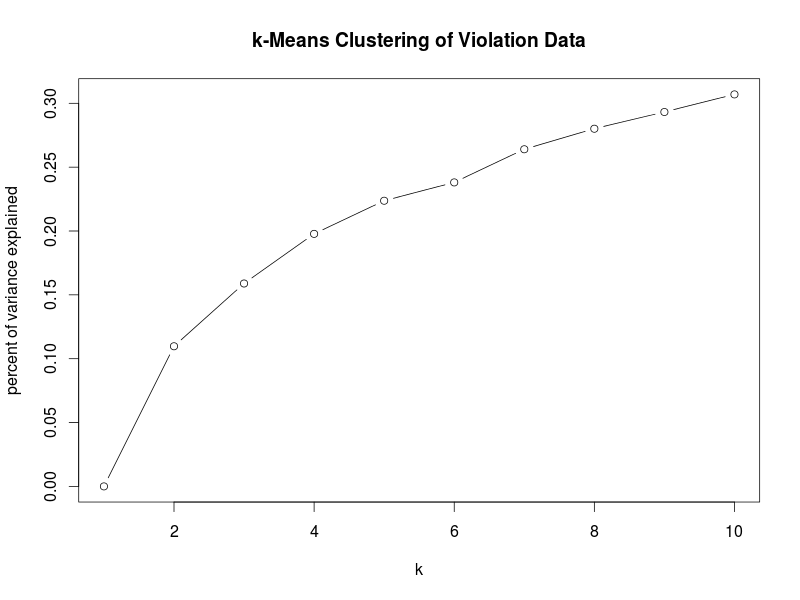
\includegraphics[width=\textwidth]{plots/elbowViolation}
	
	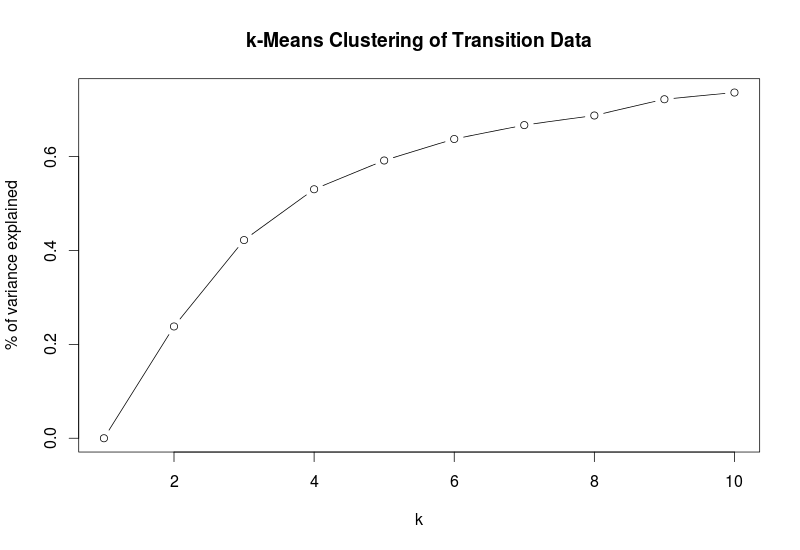
\includegraphics[width=\textwidth]{plots/elbowTransition}
\end{columns}
\end{frame}

\section{Clustering Results}
\begin{frame}{Clustering Results}
\vfill
Violation frequencies
\begin{itemize}
	\item Very sparse data
	\item Clusters don't account for much of the variance (about~25\%)
	\item Hard to interpret
\end{itemize}
\vfill
Transition matrices
\begin{itemize}
	\item Good accounting of the variance (about~60\%)
	\item Can interpret cluster centers
	\item Problems of scaling from missing data
\end{itemize}
\vfill
\end{frame}

\begin{frame}{Transition Clusters}
\vfill
$k=5$
\begin{itemize}
	\item $A \rightarrow A$, $B \rightarrow B$, and $C \rightarrow C$ dominated
	restaurants all end up clustered together
	\item Two clusters with dominant $B \rightarrow A$ transitions
	\begin{itemize}
		\item one has notable $A \rightarrow A$ and $A \rightarrow B$ transitions,
		with barely any transitions to $C$
		\item other splits evenly from $A$, when at $C$, the $C \rightarrow A$
		transition is dominant
	\end{itemize}
\end{itemize}
\vfill
\end{frame}

\begin{frame}{Transition Clusters}
\vfill
$k=9$
\begin{itemize}
	\item $A \rightarrow A$ dominated cluster is identifiable
	\item ``re-scaling'' of matrices helps make sense of centers
	\item Clusters with dominant $B \rightarrow A$ transitions still identifiable
	\begin{itemize}
		\item Third one appears that drifts down, with relatively small 
		$A \rightarrow A$ transition
	\end{itemize}
	\item Sizeable cluster with a strong $C \rightarrow A$ transition that
	then goes between $A$ and $B$ with slight chances of dropping to $C$
	\begin{itemize}
		\item Looking at unscaled version, see most of the data comes from
		transitions out of $C$
	\end{itemize}
\end{itemize}
\vfill
\end{frame}

\section{Conclusions}
\begin{frame}{Conclusion}
\vfill
Conclusions!
\vfill
Questions?
\vfill
\end{frame}

\end{document}